% Emacs settings: -*-mode: latex; TeX-master: "manual.tex"; -*-

\chapter{The component library}
\label{s:components}
This section is devoted to a description of components included in
the component library.  The component library is
maintained by the Ris\o{} group. All components were written at Ris\o\
except the chopper components in
sections~\ref{s:chopper} and~\ref{s:first_chopper} which have been
kindly contributed by Philipp Bernhardt, Lehrstuhl f\"ur
Kristallographie und Strukturphysik; and the Source\_Optimizer
(section~\ref{s:sourceoptimizer}), Monitor\_Optimizer
(section~\ref{s:monitoroptimizer}), and Monitor\_nD
(section~\ref{s:monitornd}) components which were written by Emmanuel
Farhi, Institute Laue-Langevin.
Users are encouraged to send
contributions to us for inclusion in future releases.

In the explanations of the individual components we will use
the usual symbols {\bf r} for the position $(x,y,z)$ of the particle
(unit m), and {\bf v} for 
the particle velocity $(v_x, v_y, v_z)$ (unit m/s).
Another frequently used symbol is 
the wave vector ${\bf k} = m_{\rm N} {\bf v}/\hbar$ , where
$m_{\rm N}$ is the neutron mass. {\bf k} is usually given in
\AA$^{-1}$, while neutron energies are given in meV.
In general, vectors are denoted by boldface symbols.
Subscripts "i" and "f" denotes "initial" and "final", respectively,
and are used in connection with the neutron state before and after
a scattering event.
Note that all mentioning of component geometry refer to
the local coordinate system of the individual component.

The source code for components is listed 
in Appendix~\ref{compcode}. 
The components follow the same numbering
in the Appendix as in the main text, \textit{e.g.} 
component \textbf{Arm}, subsection \ref{explain:arm},
appears in the Appendix as \ref{code:arm}.
Source code for many of the more trivial components are not included in
this manual. All sources may be found in the \verb+lib/mcstas/+
subdirectory of the McStas installation; the default is \verb+/usr/local/lib/mcstas/+.

% Emacs settings: -*-mode: latex; TeX-master: "manual.tex"; -*-

\section{Source components}
The main function of the source components is to determine a set of initial
parameters $({\bf r}, {\bf v})$, or equivalent (${\bf r}, v, \Ombold $),
for each neutron. This is done by Monte Carlo choices. 
In the current sources no polarization dependence is implemented, 
whence we let ${\bf s}=(0,0)$.

The sources to be presented in the following all make their Monte Carlo
choices on the basis of simple analytical expressions ({\em e.g.} the
energy distribution). 
More realistic sources would require that (at least) the Monte-Carlo choice
for the initial energy was made on basis of a measured,
tabulated energy spectrum.
This is planned to be implemented in a later version of \MCS .

\subsection{Source\_flat: A circular continuous source with a flat energy spectrum}
\label{sourceaim}
This component {\bf Source\_flat} is 
a simple continous source with a flat energy distribution.
The time-of-flight aspect is not relevant for this component,
so we put $t=0$ for all neutrons.

The initial neutron position is chosen randomly from within a
circle of radius $r_{\rm s}$ in the $z=0$ plane. 
This is a fair approximation
of a cylindrical cold source with the beam going out along
the cylinder axis, like the one at Ris\o .

The initial neutron velocity direction is focused within
a solid angle, defined by a rectangular target of width
$w$, height $h$, parallel to 
the $xy$ plane placed at $(0,0,z_{\rm f})$. 
A small angle approximation is used, assuming that 
$w,h \ll z_{\rm f}$.

The weight multiplier of the created neutron, $\pi_1$, is set to the
solid angle of the focusing opening divided by $4\pi$,
see discussion in \ref{s:focus}

The input parameters of {\bf Source\_flat} are the source radius, $r_{\rm s}$,
the distance to the target, $z_{\rm f}$, 
the dimensions of the target, $w$ and $h$, and
the centre and spread of the energy distribution, $E_0$ and $\Delta E$.


\subsection{Source\_flat\_lambda: A continous source with flat
  wavelength spectrum}

The component {\bf Source\_flat\_lambda} is similar to the Source\_flat
component, except that the spectrum is flat in wavelength, rather
than in energy.

The input parameters for Source\_flat\_lambda are \textit{radius} to set
the source radius in meters; \textit{dist}, \textit{xw}, and \textit{yh}
to set the focusing as for Source\_flat; and \textit{lambda\_0} and
\textit{d\_lambda} to set the range of wavelength emitted (the range
will be from $\textit{lambda\_0} - \textit{d\_lambda}$ to
$\textit{lambda\_0} + \textit{d\_lambda}$).


\subsection{Source\_flux\_lambda: A continuous source with absolute
  flux}
\label{Source_flux_lambda}

The component {\bf Source\_flux\_lambda} is a variation on the
Source\_flat\_lambda component. The only difference is the possibility
to specify the absolute flux of the source. The specified flux is used
to adjust the initial neutron weight so that the intensity in the
detectors is directly comparable to a measurement of one second on a
real source with the same flux. This also makes the simulated detector
intensities independent of the number of neutron histories simulated,
easing the comparison between different simulation runs (though of
course more neutron histories will give better statistics).

The flux~$\Phi$ is the number of neutrons emitted per second from a
one~cm$^2$ area on the source surface, with direction within a a one
steradian solid angle, and with wavelength within a one {\AA}ngstr{\o}m
interval. The total number of neutrons emitted towards a given diaframe
in one second is therefore
$$ N_{\rm total} = \Phi A \Omega \Delta\lambda $$
where $A$ is the source area, $\Omega$ is the solid angle of the
diaframe as seen from the source surface, and $\Delta\lambda$ is the
width of the wavelength interval in which neutrons are emitted (assuming
a uniform wavelength spectrum). If $N_{\rm sim}$ denotes the number of
neutron histories to simulate, the initial neutron weight $p_0$ must be set to
$$ p_0 = \frac{N_{\rm total}}{N_{\rm sim}} = 
    \frac{\Phi}{N_{\rm sim}} A \Omega \Delta\lambda $$

The input parameters for Source\_flux\_lambda are \textit{radius} to set
the source radius in meters; \textit{dist}, \textit{xw}, and \textit{yh}
to set the focusing as for Source\_flat; \textit{lambda\_0} and
\textit{d\_lambda} to set the range of wavelength emitted (the range
will be from $\textit{lambda\_0} - \textit{d\_lambda}$ to
$\textit{lambda\_0} + \textit{d\_lambda}$); and \textit{flux} to set the
source flux in units of ${\rm cm}^{-2} {\rm st}^{-1} \textit{\AA}$.


\subsection{Source\_div: A divergent source}

{\bf Source\_div} is a rectangular source which emits a
beam of a certain divergence around the main exit direction
(the direction of the $z$ axis).
The beam intensity and divergence are uniform over
the whole of the source, and the energy distribution
of the beam is uniform.

This component may be used as a simple model of the
beam profile at the end of a guide or at the sample
position.

The input parameters for Source\_div are the source dimensions
$w$ and $h$ (in m), the divergencies $\delta_h$ and $\delta_v$ (FWHM in degrees), 
and the mean energy $E_0$ and the energy spread $dE$ (both in meV).
The neutron energy range is $(E_0-dE; E_0+dE)$. 


\subsection{Moderator: A time-of-flight source}
The simple time-of-flight source component {\bf Moderator} resembles
the source component {\bf Source\_flat} described in \ref{sourceaim}.
Like {\bf Source\_flat}, {\bf Moderator} is circular and focuses
on a rectangular target. Further, the initial velocity is chosen
with a linear distribution within an interval, defined by the
minimum and maximum energies, $E_0$ and $E_1$,
respectively.

The initial time of the neutron is determined on basis of a 
simple heuristical model for the time dependence of the 
neutron intensity from a time-of-flight source.
For all neutron energies, the flux decay is assumed to be exponential,
\begin{equation}
\Psi(E,t) = \exp(-t/\tau(E)) ,
\end{equation}
where the decay constant is given by
\begin{equation}
\tau(E) = \left\{ 
\begin{array}{cc}
 \tau_0                               & ; E<E_c \\
 \tau_0 / [ 1 + (E-E_c)^2/\gamma^2 ]  & ; E \geq E_c
\end{array}
\right.
\end{equation}

The input parameters for {\bf Moderator} are the source radius, $r_{\rm s}$,
the minimum and maximum energies, $E_0$ and $E_1$ (in meV),
the distance to the target, $z_{\rm f}$, the dimensions of the target,
$w$ and $h$, and the decay parameters 
$\tau_0$ (in $\mu$s), $E_c$, and $\gamma$ (both in meV).


% Emacs settings: -*-mode: latex; TeX-master: "manual.tex"; -*-

\section{Source\_adapt: A neutron source with adaptive importance sampling}
\label{s:Source_adapt}
\label{s:source-adapt}
\index{s:source-adapt}
\index{Optimization}

The {\bf Source\_adapt} component is a neutron source that uses adaptive
importance sampling to improve the efficiency of the simulations. It
works by changing on-the-fly the probability distributions from which
the initial neutron state is sampled so that samples in regions that
contribute much to the accuracy of the overall result are preferred over
samples that contribute little. The method can achieve improvements of a
factor of ten or sometimes several hundred in simulations where only a
small part of the initial phase space contains useful neutrons.
On the other side, a warning is in place here regarding potential wrong results using optimization techniques (see section \ref{s:optim} of the \MCS\ user manual). It is highly recommanded in any case to benchmark 'optimized' simulations against non-optimized ones, checking that obtained results are the same, but hopefully with a much improved statistics.

The physical characteristics of the source are similar to those of
Source\_flat (see section~\ref{sourceaim}). The source is a thin
rectangle in the $X$-$Y$ plane with a flat energy spectrum in a
user-specified range. The flux per area per steradian per
{\AA}ngstr{\o}m per second is specified by the user; the total weight of
neutrons emitted from the source will then be the same irrespectively of
the number of neutron histories simulated, corresponding to one second
of measurements.

The initial neutron weight is given by (see
section~\ref{Source_flux_lambda} for details)
$$ p_0 = \frac{N_{\rm total}}{N_{\rm sim}} =
    \frac{\Phi}{N_{\rm sim}} A \Omega \Delta\lambda $$
Here $\Delta\lambda$ is the total wavelength range of the source; since
the spectrum is flat in energy (but not in wavelength), the flux
will actually be different for different energies. A later version of
this component will probably adapt (in a backward-compatible way) a more
sensible way to specify the flux. For now, an energy or wavelength
monitor (see sections~\ref{s:e_monitor} and~\ref{s:L_monitor}) placed
just after the source will show the actual energy-dependent flux.


\subsection{The adaption algorithm}

The adaptive importance sampling works by subdividing the initial
neutron phase space into a number of equal-sized bins. The division is
done on the three dimensions of energy, horizontal position, and
horizontal divergence, using $N_{\rm eng}$, $N_{\rm pos}$, and $N_{\rm
  div}$ number of bins in each dimension, respectively. The total number
of bins is therefore
$$
N_{\rm bin} = N_{\rm eng} N_{\rm pos} N_{\rm div}
$$
Each bin $i$ is assigned a sampling weight $w_i$; the probability of
emitting a neutron within bin $i$ is
$$
P(i) = \frac{w_i}{\sum_{j=1}^{N_{\rm bin}} w_j}
$$
In order to avoid false learning, the sampling weight of a bin is
kept larger than $w_{\rm min}$, defined as
$$
w_{\rm min} = \frac{\beta}{N_{\rm bin}}\sum_{j=1}^{N_{\rm bin}}w_j,\qquad
    0 \leq \beta \leq 1
$$
This way a (small) fraction $\beta$ of the neutrons are sampled
uniformly from all bins, while the fraction $(1 - \beta)$ are sampled in an adaptive way.

Compared to a uniform sampling of the phase space (where the probability
of each bin is $1/N_{\rm bin}$), the neutron weight
must be adjusted by the amount
$$
\pi_i = \frac{1/N_{\rm bin}}{P(i)} =
    \frac{\sum_{j=1}^{N_{\rm bin}} w_j}{N_{\rm bin} w_i}
$$

In order to set the criteria for adaption, the Adapt\_check component is
used (see section~\ref{s:adapt_check}). The source attemps to sample
only from bins from which neutrons are not absorbed prior to the
position in the instrument at which the Adapt\_check component is
placed. Among those bins, the algorithm attemps to minimize the variance
of the neutron weights at the Adapt\_check position. Thus bins that
would give high weights at the Adapt\_check position are sampled more
often (lowering the weights), while those with low weights are sampled
less often.

Let $\pi = p_1/p_0$ denote the ratio between the neutron weight $p_1$ at
the Adapt\_check position and the initial weight $p_0$ just after the
source. For each bin, the component keeps track of the sum $\psi$ of
$\pi$'s as well as of the total number of neutrons $n_i$ from that
bin. The average weight at the Adapt\_source position of bin $i$ is thus
$\psi_i/n_i$.

We now distribute a total sampling weight of $\beta$ uniformly
among all the bins, and a total weight of $(1 - \beta)$ among bins in
proportion to their average weight $\psi_i/n_i$ at the Adapt\_source
position:
$$
w_i = \frac{\beta}{N_{\rm bin}} +
    (1-\beta) \frac{\psi_i/n_i}{\sum_{j=1}^{N_{\rm bins}} \psi_j/n_j}
$$
After each neutron event originating from bin $i$, the sampling weight $w_i$
is updated.

This basic idea can be improved with a small modification. The problem
is that until the source has had the time to learn the right sampling
weights, neutrons may be emitted with high neutron weights (but low
probability). These low probability neutrons may account for a large fraction of
the total intensity in detectors, causing large variances in the
result. To avoid this, the component emits early neutrons with a lower
weight, and later neutrons with a higher weight to compensate. This way
the neutrons that are emitted with the best adaption contribute the most
to the result.

The factor with which the neutron weights are adjusted is given by a
logistic curve
\begin{equation}
  F(j) = C\frac{y_0}{y_0 + (1 - y_0) e^{-r_0 j}}
\end{equation}
where $j$ is the index of the particular neutron history, $1 \leq j
\leq N_{\rm hist}$. The constants $y_0$, $r_0$, and $C$ are given by
\begin{eqnarray}
  y_0 &=& \frac{2}{N_{\rm bin}} \\
  r_0 &=& \frac{1}{\alpha}\frac{1}{N_{\rm hist}}
     \log\left(\frac{1 - y_0}{y_0}\right) \\
  C &=& 1 + \log\left(y_0 + \frac{1 - y_0}{N_{\rm hist}}
     e^{-r_0 N_{\rm hist}}\right)
\end{eqnarray}
The number $\alpha$ is given by the user and specifies (as a fraction
between zero and one) the point at which the adaption is considered
good. The initial fraction $\alpha$ of neutron histories are emitted
with low weight; the rest are emitted with high weight:
$$ p_0(j) =
    \frac{\Phi}{N_{\rm sim}} A \Omega \Delta\lambda
    \frac{\sum_{j=1}^{N_{\rm bin}} w_j}{N_{\rm bin} w_i}
    F(j)
$$
The choice of the constants $y_0$, $r_0$, and $C$ ensure that
$$
\int_{t=0}^{N_{\rm hist}} F(j) = 1
$$
so that the total intensity over the whole simulation will be correct

Similarly, the adjustment of sampling weights is modified so that the
actual formula used is
$$
w_i(j) = \frac{\beta}{N_{\rm bin}} +
    (1-\beta) \frac{y_0}{y_0 + (1 - y_0) e^{-r_0 j}}
     \frac{\psi_i/n_i}{\sum_{j=1}^{N_{\rm bins}} \psi_j/n_j}
$$

\subsection{The implementation}

\component{Source\_adapt}{K. Nielsen}{$x_{min}$, $x_{max}$, $y_{min}$, $y_{max}$, $E0$, $dE$, dist, $xw$, $yh$, $Phi$}{$\alpha$, $\beta$ (plenty, default values are ok)}{not fully validated}

The heart of the algorithm is a discrete distribution $p$. The
distribution has $N$ \emph{bins}, $1\ldots N$. Each bin has a value
$v_i$; the probability of bin $i$ is then $v_i/(\sum_{j=1}^N v_j)$.

Two basic operations are possible on the distribution. An \emph{update}
adds a number $a$ to a bin, setting $v_i^{\rm new} = v_i^{\rm old} +
a$. A \emph{search} finds, for given input $b$, the minimum $i$ such
that
$$ b \leq \sum_{j=1}^{i} v_j. $$
The search operation is used to sample from the distribution p. If $r$
is a uniformly distributed random number on the interval
$[0;\sum_{j=1}^N v_j]$ then $i = {\rm search}(r)$ is a random number
distributed according to $p$. This is seen from the inequality
$$ \sum_{j=1}^{i-1} v_j < r \leq \sum_{j=1}^{i} v_j, $$
from which $r \in [\sum_{j=1}^{i-1} v_j; v_i + \sum_{j=1}^{i-1} v_j]$
which is an interval of length $v_i$. Hence the probability of $i$ is
$v_i/(\sum_{j=1}^N v_j)$.
The update operation is used to
adapt the distribution to the problem at hand during a simulation. Both
the update and the add operation can be performed very efficiently; how
this is achieved will be described elsewhere.

The input parameters for Source\_adapt are
\textit{xmin}, \textit{xmax}, \textit{ymin}, and
\textit{ymax} in meters to set the source dimensions;
\textit{dist}, \textit{xw}, and \textit{yh}
to set the focusing as for Source\_flat (section~\ref{sourceaim}); \textit{E0} and
\textit{dE} to set the range of energies emitted, in meV (the range
will be from $\textit{E0} - \textit{dE}$ to
$\textit{E0} + \textit{dE}$); flux to set the source flux $\Phi$ in ${\rm
  cm}^{-2} {\rm st}^{-1} \textit{\AA} {\rm s}^{-1}$;
$N_{\rm eng}$, $N_{\rm pos}$, and $N_{\rm
  div}$ to set the number of bins in each dimensions; \textit{alpha} and
\textit{beta} to set the parameters $\alpha$ and $\beta$ as described
above; and \textit{filename} to give the name of a file in which to
output the final sampling destribution.

A good general-purpose value for $\alpha$ and $\beta$ is $\alpha = \beta
= 0.25$. The number of bins to choose will depend on the
application. More bins will allow better adaption of the sampling, but
will require more neutron histories to be simulated before a good
adaption is obtained. The output of the sampling distribution is only
meant for debugging, and the units on the axis are not necessarily
meaningful. Setting the filename to \verb+NULL+ disables the output of
the sampling distribution.

As an alternative, you may use the Source\_Optimizer component (see section \ref{source-optimizer}).


\input{Source_Optimizer}

% Emacs settings: -*-mode: latex; TeX-master: "manual.tex"; -*-

\section{Simple optical components:
Arms, slits, collimators, filters}
Below we list a number of simple optical components 
which require only a minimum of explanation.

\subsection{Arm: The generic component}
\label{explain:arm}
The component {\bf Arm} is empty; is resembles an optical bench
and has no effect on the neutron.
The function of this component is only to set up a local frame of
reference within the instrument definition. Other components of the
same arm/optical bench may then be
positioned relative to the arm component
using the \MCS\ meta-language.
The use of arm components in the instrument definitions
is not required but is recommended for clarity.

{\bf Arm} has no input parameters.
For more about the use of this component, see the 
sample instrument definitions listed in Appendix \ref{instcode}.


\subsection{Slit: The rectangular slit}
\label{slit}
The component {\bf Slit} is a very simple construction.
It sets up a rectangular opening at $z=0$, and propagates the neutrons 
onto the plane of this rectangle by the kernel call PROP\_Z0.

Neutrons within the slit opening are unaffected, 
while all other neutrons
(no matter how far from the opening their paths intersect the plane)
are discarded by the kernel call ABSORB.
By this simplification, some neutrons contributing to the background
in a real experiment will be neglected. 
These are the ones that scatter off the inner side
of the slit, penetrates the slit material, 
or that clear one of the outer edges of the slit.

The input parameters of {\bf Slit} are the four coordinates,
$(x_{\rm min}, x_{\rm max}, y_{\rm min}, y_{\rm max})$
defining the opening of the rectangle.

\subsection{Circular\_slit: The circular slit}
The component {\bf Circular\_slit} defines a circle in the $z=0$ plane,
centered in the origin. In analogy with {\bf Slit},
neutrons are propagated to this plane, and those which intersect
the plane outside the circle are ABSORB'ed.

The only input parameter of {\bf Circular\_slit} is
the radius, $r$, of the circle.

\subsection{Beamstop\_rectangular: The rectangular beam stop}
\label{s:Beamstop_rectangular}
The component {\bf Beamstop\_rectangular} models a thin, infinitely
absorbing rectangle in the $X$-$Y$ plane, centered on the origin. The
input parameters are \textit{xmin}, \textit{xmax}, \textit{ymin}, and
\textit{ymax} defining the edges of the slit in meters.


\subsection{Beamstop\_circular: The circular beam stop}
\label{s:Beamstop_circular}
The component {\bf Beamstop\_circular} models a thin, infinitely
absorbing circular disk in the $X$-$Y$ plane, centered on the origin. It
takes a single input parameter \textit{radius} to define the circle
radius in meters.


\subsection{Soller: The simple Soller blade collimator}
The component {\bf Soller} defines two rectangular openings
like the one in {\bf Slit}. Neutrons not clearing both these
openings are ABSORB'ed, see the discussion in \ref{slit}.
The collimating effect is taken care of by employing an ideal
triangular transmission through the collimator, as explained below.
For a more detailed Soller collimator simulation the Channeled\_guide
component can be employed, see section~\ref{s:channeled_guide}.

Let the collimation angle be $\delta = \tan^{-1}(d/L)$,
where $L$ is the length of the collimator
and $d$ is the distance between the blades,
and let $\phi$ be the divergence angle between the 
neutron path and a vertical plane along the collimator axis, 
see Fig.~\ref{f:collimator}. Neutrons with a large 
divergence angle $|\phi| \geq \delta$ will always
hit at least one collimator blade and will thus be absorbed.
For smaller divergence angles, $|\phi| < \delta$, the fate of the
neutron depends on its exact entry point.
Assuming that a typical collimator has many blades, the
absolute position of each blade perpendicular to the collimator axis
is somewhat uncertain (and also unimportant).
A simple statistical consideration now shows that the transmission
probability is $T = 1-\tan|\phi|/\tan\delta$.

\begin{figure}
  \begin{center}
    \psfrag{xmin}[c][c]{$x_{\rm min}$}
    \psfrag{xmax}[c][c]{$x_{\rm max}$}
    \psfrag{ymin}[c][c]{$y_{\rm min}$}
    \psfrag{ymax}[c][c]{$y_{\rm max}$}
    \psfrag{delta}[c][c]{$\delta$}
    \includegraphics[width=0.9\textwidth]{figures/collimator.eps}
  \end{center}
\caption{The geometry of a simple Soller blade collimators:
The real Soller collimator, seen from the top (left), 
and a sketch of the component {\bf Soller} (right).
The symbols are defined in the text.}
\label{f:collimator}
\end{figure}

We simulate the collimator by transmitting all neutrons with
$|\phi| < \delta$, but adjusting their weight with the amount
\begin{equation}
\pi_i = T = 1-\tan|\phi|/ \tan\delta ,
\end{equation}
while all others are discarded by the kernel call ABSORB.

The input parameters for {\bf Soller} are the coordinates
$(x_{\rm min}, x_{\rm max}, y_{\rm min}, y_{\rm max})$,
defining the identical entry and exit apertures, 
the length, $l$, between the slits, 
and the collimator divergence $\delta$.
If $\delta=0$, the collimating effect is disabled,
so that $\pi_i = 1$ whenever the neutron clears the two apertures.

\subsection{Filter: A transmission filter}
A neutron transmission filter act in much of the same way as two
identical slits, one after the other.
The only difference is that the transmission of the filter
varies with the neutron energy.

In the simple component {\bf Filter},
we have not tried to simulate the details of the transmission
process (which includes absorption, incoherent scattering,
and Bragg scattering in a polycrystalline sample, {\em e.g.} Be).
Instead, the transmission is parametrised to be
$\pi_i=T_0$ when $E \leq E_{\rm min}$, $\pi_i=T_1$ when $E \geq E_{\rm max}$,
and linearly interpolated between the two values
in the intermediate interval.
\begin{equation}
\pi_i = \left\{ \begin{array}{lc}
 T_0  & E \leq E_{\rm min} \\
 T_1 + (T_0-T_1) \frac{E_{\rm max}-E}{E_{\rm max}-E_{\rm min}}
 & E_{\rm min} < E < E_{\rm max} \\
 T_1  & E_\geq E_{\rm max} \\
\end{array} \right.
\end{equation}
If $T_1=0$, the neutrons with $E>E_{\rm max}$ are ABSORB'ed.

The input parameters are the four slit coordinates, 
$(x_{\rm min}, x_{\rm max}, y_{\rm min}, y_{\rm max})$,
the distance, $l$, between the slits, and the transmission parameters 
$T_0$, $T_1$, $E_{\rm min}$, and $E_{\rm max}$. 
The energies are given in meV.

% Emacs settings: -*-mode: latex; TeX-master: "manual.tex"; -*-

\section{Advanced optical components: mirrors and guides}

This section describes advanced neutron optical
components such as supermirrors and guides.
The first subsection, however, contains 
only a description of the reflectivity of a supermirror.

\subsection{Mirror reflectivity}
\label{s:mirrorreflect}
To compute the reflectivity of the supermirrors, we use an empirical
formula derived from experimental data (see figure~\ref{f:reflectivity}). 
The reflectivity is given by the following formula
\begin{equation}
  R = \left\{
    \begin{array}{ll}
      R_0 & \textrm{if $Q \leq Q_{\rm c}$} \\
      \frac{1}{2}R_0(1 - \tanh[(Q - m Q_{\rm c})/W])(1-\alpha(Q-Q_{\rm c}))
         & \textrm{if $Q > Q_{\rm c}$}
    \end{array}
  \right.
\end{equation}

\begin{figure}
  \begin{center}
    \includegraphics[width=0.6\textwidth]{figures/supermirror.eps}
  \end{center}
\caption{A typical reflectivity curve for a supermirror,
Eq.~(\protect\ref{e:reflectivity}).}
\label{f:reflectivity}
\end{figure}
Here $Q$ is the length of the scattering vector (in \AA$^{-1}$)
defined by
\begin{equation} \label{e:reflectivity}
Q = |{\bf k}_{\bf i} - {\bf k}_{\bf f}| 
  = \frac{m_{\rm n}}{\hbar} |{\bf v}_{\bf i} - {\bf v}_{\bf f}|, 
\end{equation}
$m_{\rm n}$ being the neutron mass. 
The value $m$ is a parameter determined by the mirror materials,
the bilayer sequence, and the number of bilayers.
As can be seen, $R=R_0$ for $Q < Q_{\rm c}$, which is the
critical scattering wave vector for a single layer of the mirror
material. At higher values of $Q$, the reflectivity starts falling
linearly with a slope $\alpha$ until a cut-off at $Q = m Q_{\rm c}$. 
The width of the cut-off is denoted $W$. For the curve in
figure~\ref{f:reflectivity}, the values are
$$ m=4 \qquad R_0=1 \qquad Q_{\rm c} = 0.02\mbox{ \AA}^{-1} \qquad
   \alpha = 6.49\mbox{ \AA} \qquad W=1/300\mbox{ \AA}^{-1} $$
As a special case, if $m=0$ then the reflectivity is zero for all $Q$,
   \textit{ie.} the surface is completely absorbing.

In the components, the neutron weight is adjusted with the amount $\pi_i = R$. 
To avoid spending large amounts of computation time on very low-weight
neutrons, neutrons for which the reflectivity is lower than about
$10^{-10}$ are ABSORB'ed.

\subsection{Mirror: The single mirror}

The component {\bf Mirror} 
models a single rectangular neutron mirror plate. It can
be used to \textit{e.g.}~assemble a complete neutron guide by putting multiple
mirror components at appropriate locations and orientations in the
instrument definition, much like a real guide is build from individual
mirrors.

The mirror is assumed to lie in the first quadrant of the
$x$-$y$ plane, with one corner at $(0,0,0)$. 
If the neutron trajectory intersects the mirror plate, it is
reflected, otherwise it is left untouched. Since the mirror lies in the
$x$-$y$ plane, an incoming neutron with velocity 
${\bf v}_{\rm i} = (v_x,v_y,v_z)$
is reflected with velocity ${\bf v}_{\rm f} = (v_x,v_y,-v_z)$. 
The computation of the reflectivity is handled as detailed in
section~\ref{s:mirrorreflect}.

The input parameters of this component are
the rectangular mirror dimensions $(l, h)$
and the values of $R_0, m, Q_c, W$, and $\alpha$ for the mirror.


\subsection{Guide: The guide section}

The component {\bf Guide} 
models a guide tube consisting of four flat mirrors. The
guide is centered on the $z$ axis with rectangular entrance and exit
openings parallel to the $x$-$y$ plane. The entrance has the dimensions
$(w_1,h_1)$ and placed at $z=0$. The exit is of dimensions $(w_2,h_2)$
and is placed at $z=l$ where $l$ is the guide length. See
figure~\ref{f:guide}. Neutrons not clearing the guide entrance are
ABSORB'ed. For a more general guide simulation, see the Channeled\_guide
component in section~\ref{s:channeled_guide}.

\begin{figure}
  \begin{center}
    \includegraphics[width=0.9\textwidth]{figures/guide1.eps}
  \end{center}
\caption{The geometry used for the guide component.}
\label{f:guide}
\end{figure}

For computations on the guide geometry, we define the planes of the four
guide sides by giving their normal vectors (pointing into the guide)
and a point lying in the plane:
$$
\begin{array}{rclcrcl}
{\bf n}^v_1 &=& (l, 0, {(w_2 - w_1) / 2})
     & & {\bf O}^v_1 &=& (- w_1 / 2, 0, 0) \\
{\bf n}^v_2 &=& (-l, 0, {(w_2 - w_1) / 2})
     & & {\bf O}^v_2 &=& (w_1 / 2, 0, 0) \\
{\bf n}^h_1 &=& (0, l, {(h_2 - h_1) / 2})
     & & {\bf O}^h_1 &=& (0, - h_1 / 2, 0) \\
{\bf n}^h_2 &=& (0, -l, {(h_2 - h_1) / 2})
     & & {\bf O}^h_2 &=& (0, h_1 / 2, 0) \\
\end{array}
$$
In the following, we refer to an arbitrary guide side by its origin
{\bf O} and normal {\bf n}.

With these definitions, the time of intersection of the neutron with a
guide side can be computed by considering the projection onto the
normal:
\begin{equation} 
t_1 = {({\bf O} - {\bf r}_0) \cdot {\bf n} \over {\bf v} \cdot {\bf n}} 
\end{equation}
For a neutron that leaves the guide through the guide exit we have
\begin{equation}
t_2 = {l - z_0 \over v_z} 
\end{equation}
To compute the interaction of the neutron
with the guide, the neutron is initially propagated to the $z = 0$ plane of the
guide entrance. If it misses the entrance, it is ABSORB'ed. Otherwise,
we repeatedly compute the time of intersection with the
four mirror sides and the guide exit. The smallest positive $t$ thus
found gives the time of the next intersection with the guide (or in the
case of the guide exit, the time when the neutron leaves the guide). The
neutron is propagated to this point, the reflection from the side is
computed and the process is repeated until the neutron leaves the guide.

The reflected velocity ${\bf v}_{\rm f}$ of the neutron with incoming velocity
${\bf v}_{\rm i}$ is computed by the formula
\begin{equation}
 {\bf v}_{\rm f} = 
  {\bf v}_{\rm i} 
   - 2{{\bf n} \cdot {\bf v}_{\rm i} \over {|{\bf n}|^2}} {\bf n}
\end{equation}
This expression is arrived at by again considering the projection onto
the mirror normal (see figure~\ref{f:guidereflect}). The reflectivity of the
mirror is taken into account as explained in section~\ref{s:mirrorreflect}.

\begin{figure}
  \begin{center}
    \includegraphics[width=0.5\textwidth]{figures/guide2.eps}
  \end{center}
\caption{Neutron reflecting from mirror. ${\bf v}_{\rm i}$ and 
${\bf v}_{\rm f}$ are the initial and final velocities, respectively,
and {\bf n} is a vector normal to the mirror surface.}
\label{f:guidereflect}
\end{figure}

There are a few optimizations possible here to avoid redundant
computations. Since the neutron is always inside the guide during the
computations, we always have 
$({\bf O} - {\bf r}_0) \cdot {\bf n} \leq 0$. 
Thus $t \leq 0$ if ${\bf v} \cdot {\bf n} \geq 0$, so in this case
there is no need to actually compute $t$. Some redundant computations
are also avoided by utilizing symmetry and the fact that many
components of {\bf n} and {\bf O} are zero.

The input parameters of this component are
the opening sizes of the entry and exit point of the
guide, $(w_1, h_1)$ and $(w_2, h_2)$, respectively,
the guide length, $l$,
and the values of $R_0, m, Q_c, W$, and $\alpha$ for the mirror.


\subsection{Channeled\_guide: A guide section component with multiple channels}
\label{s:channeled_guide}

The component Channeled\_guide is a more flexible variation of the Guide
component described in the previous section. It allows the specification
of different supermirror parameters for the horizontal and vertical
mirrors, and also implements guides with multiple channels as used in
neutron bender devices. By setting the $m$ value of the supermirror
coatings to zero, nonreflecting walls are
simulated; this may be used to simulate a Soller collimator.

The channel walls are assumed to be infinitely absorbing. The
implementation is basen on that of the Guide component. Initially, the
channel which the neutron will enter is computed. The $x$ coordinate is
then shifted so that the channel can be simulated as a single instance
of the Guide component. Finally the coordinates are restored when the
neutron exits the guide or is absorbed.

The input parameters are \textit{w1}, \textit{h1}, \textit{w2},
\textit{h2}, and \textit{l} to set the guide dimensions in meters as for
the Guide component (entry window, exit window, and length); \textit{k}
to set the number of channels; \textit{d} to set the thickness of the
channel walls, in meters; and \textit{R0}, \textit{W}, \textit{Qcx},
\textit{Qcy}, \textit{alphax}, \textit{alphay}, \textit{mx}, and \textit{my} to
set the supermirror parameters as described above (the names with \textit{x}
denote the vertical mirrors, and those with \textit{y} denote the horizontal
ones).

% Emacs settings: -*-mode: latex; TeX-master: "manual.tex"; -*-

\section{Chopper: The disc chopper}
\label{s:chopper}
\index{Optics!Disc chopper}

\component{Chopper}{Phillipp Bernhardt}{$w$, $R$, $f$, $n$, $\phi$}{IsFirst, $n_{\rm pulse}$}{}

To cut a continuous neutron beam into short pulses, or to control
the pulse shape from a pulsed source, one can use a disc
chopper (see figure~\ref{f:chopper1}). This is a fast rotating disc with the
rotating axis parallel to the neutron beam. The disk consists of neutron
absorbing materials. To form the pulses the disk has openings through which
the neutrons can pass.

\begin{figure}[ht]
\includegraphics[width=1.0\linewidth]{figures/Chopper.eps}
\caption{disc chopper\label{f:chopper1}}
\end{figure}

Component {\bf Chopper} has $n$ openings, which are
symmetrically positioned on the disc. You can set the direction of
rotation, which allows to simulate double choppers. You can also define
the phase by setting the time at which one slit is positioned at the
top. The sides of the slits are pointing towards the center of the disc.
The thickness of the disc is neglected.  There is no parameter for the
size of the slits in the radial direction;
use e.g. a {\bf Slit} component in front of the chopper.

Using a rectangular shaped beam with nearly the same
size as the slit, yields an almost triangular shaped
transmission curve (see figure~\ref{f:chopper2}).

\begin{figure}[ht]
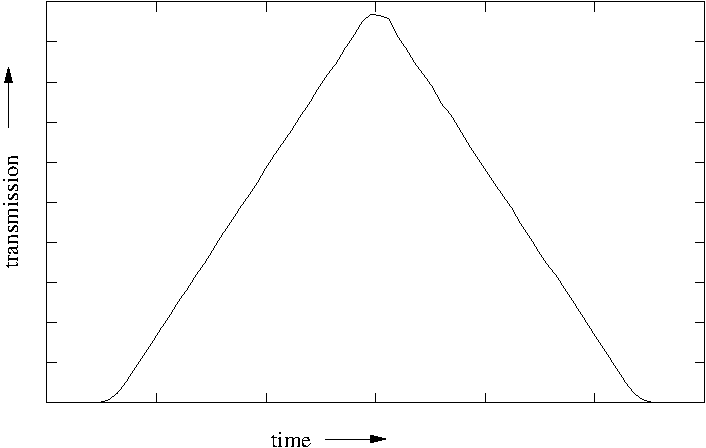
\includegraphics[width=1.0\linewidth]{figures/tracho.eps}
\caption{example transmission curve for the disc chopper\label{f:chopper2}}
\end{figure}

When simulating the chopping of a continuous beam,
most of the neutrons could easily be lost.
To improve efficiency, one can set the flag \verb+IsFirst+, which will
allow every neutron ray to pass the {\bf Chopper}, but modify the
time, $t$, to a time at which it is possible to pass.
This can also be used with TOF-instruments, which often
define the starting time of the neutrons at
the position of the first chopper.
Of course, there should be only one ``first chopper'' in
any simulation.
To simulate frame overlap from a ``first chopper'', one can specify
the number of frames to study by the parameter $n_{\rm pulse}$.
\input{detector}
% Emacs settings: -*-mode: latex; TeX-master: "manual.tex"; -*-

\section{Bragg scattering single crystals, monochromators}

In this class of components, we are concerned with elastic Bragg
scattering from single crystals. The Mosaic\_anisotropic component
models a thin mosaic crystal with a single scattering vector
perpendicular to the surface. It is a replacement for the Monochromator
component from previous releases; it uses a better algorithm that works
in some cases where the old component would give wrong results. The
Mosaic\_simple component is similar, but has an isotropic mosaic and
allows a scattering vector that is not perpendicular to the surface. The
Single\_crystal component is a general single crystal sample that allows
the input of an arbitrary unit cell and a list of structure factors, and
also allows anisotropic mosaic and $\Delta d/d$ lattice space variation.

\input{Mosaic_simple.tex}
\subsection{Mosaic\_anisotropic: The crystal with anisotropic mosaic}

The component {\bf Mosaic\_anisotropic} is a modified version of the
Mosaic\_simple component, intended to replace the Monocromator component
from previous releases. It restricts the scattering vector to be
perpendicular to the crystal surface, but extends the Mosaic\_simple
component by allowing different mosaics in the horizontal and vertical
direction.

The code is largely similar to that for Mosaic\_simple, and the
documentation for the latter should be consulted for details. The
differences are mainly due to two reasons:
\begin{itemize}
\item Some simplifications have been done since two of the components of
  the scattering vector are known to be zero.
\item The computation of the Gaussian for the mosaic is done done using
  different mosaics for the two axes.
\end{itemize}

The input parameters for the component Mosaic\_anisotropic are
\textit{zmin}, \textit{zmax}, \textit{ymin}, and \textit{ymax} to define
the size of the crystal (in meters); \textit{mosaich} and \textit{mosaicv} to define
the mosaic (in minutes of arc); \textit{r0} to define the reflectivity
(no unit); and \textit{Q} to set the length of the scattering vector (in
$\mbox{\AA}^{-1}$).

\input{Single_crystal.tex}

\subsection{Monochromator: The monochromator crystal}
The component {\bf Monochromator} is obsolete as from McStas version
1.2. Use the component {\bf Mosaic\_anisotropic} instead.

\input{powder}
% Emacs settings: -*-mode: latex; TeX-master: "manual.tex"; -*-

\section{Inelastic scattering kernels}
\label{s:inelastic}

In this section, samples with inelastic scattering are
described. Currently, only a single sample is available that scatters
uniformly in $({\bf Q}, \omega)$ and is used for computing resolution
functions in tripple-axis instruments.

\subsection{Res\_sample: A uniform scatterer for resolution calculation}
\label{s:res_sample}

The component \textbf{Res\_sample} models an inelastic sample that
scatters completely homogeneous in position and energy; regardless of
the state of the incoming neutron, all directions and energies for the
scattered neutron have the same probability. This clearly does not
correspond any physically realizable samples, but the component is very
useful for computation of the resolution function and may also be used
for test and debugging purposes. The component is designed to be used
together with the \textbf{Res\_monitor} component, described in
section~\ref{s:res_monitor}.

The shape of the sample is either a hollow cylinder (like the vanadium
sample described in section~\ref{s:v_sample}) or a rectangular box. The
hollow cylinder shape is specified with inner and outer radius \textit{radius\_i}
and \textit{radius\_o} and height \textit{h}. If \textit{radius\_o} is
negative, the shape is instead a box of width \textit{radius\_i} along
the X axis, height \textit{h}, and thickness $-\textit{radius\_o}$ along the
Z axis, centered on the Z axis and with the front face in the X-Y
plane. See figure~\ref{f:res_sample}.\par
%
\begin{figure}[htbp]
  \begin{center}
        \psfrag{ri}[c][c]{\textit{radius\_i}}
        \psfrag{ro}[c][c]{\textit{radius\_o}}
        \psfrag{h}[c][c]{\textit{h}}
        \psfrag{bri}[c][c]{\textit{radius\_i}}
        \psfrag{bro}[c][c]{$-\textit{radius\_o}$}
        \psfrag{bh}[c][c]{\textit{h}}
        \psfrag{X}[c][c]{\textit{X}}
        \psfrag{Y}[c][c]{\textit{Y}}
        \psfrag{Z}[c][c]{\textit{Z}}
        \includegraphics[width=0.9\textwidth]{figures/res_sample.eps}
    \caption{The two possible shapes of the \textbf{Res\_sample} component.}
    \label{f:res_sample}
  \end{center}
\end{figure}
%
The component only propagates the neutrons that are scattered; neutrons
that would pass through or miss the sample are absorbed. There is no
modeling of the cross section of the sample, secondary extinction
\textit{etc.}; the scattering probability is proportional to the neutron
flight path length inside the sample, with the constant of
proportionality arbitrarily set to $1/(2|\textit{radius\_o}|)$. The
reason for this is that the component is designed for computing the resolution
function of an instrument, including the sample size but independent of
any sample properties such as scattering and absorbtion cross sections.

The point of scattering in the sample is chosen at a random position
along the neutron flight path inside the sample, and the scattered
neutron is given a random energy and direction. The energy is selected in
a user-specified interval $[E_0-\Delta E; E_0+\Delta E]$ which must be
chosen large enough to cover all interesting neutrons, but preferably
not excessively large for reasons of efficiency. Similarly, the
direction is chosen in a user-specified range; the range is such that a
sphere of given center and radius is fully illuminated.

A special feature, used when computing resolution functions, is that the
component stores complete information about the scattering event in the
output parameter \textit{res\_struct}. The information includes initial
and final wave vectors, the coordinates of the scattering point, and the
neutron weight after the scattering event. From this information the
scattering parameters $({\bf Q}_i, \omega_i)$ for every scattering event
$i$ may be recorded and used to compute the resolution function of an
instrument, as explained below. For an example of how to use the
information in the output parameter, see the description of the
\textbf{Res\_monitor} component in section~\ref{s:res_monitor}.

The input parameters to the \textbf{Res\_sample} components are the
sample dimensions \textit{radius\_i}, \textit{radius\_o}, and
\textit{h}, all in meters; the center of the scattered energy range
\textit{E0} and the energy spread \textit{dE} in meV; and the target
sphere position in the local coordinate system \textit{target\_x},
\textit{target\_y}, \textit{target\_z}, and radius \textit{focus\_r}, in
meters. The only output parameter is \textit{res\_struct} containing
information about the scattering event, with all vectors given in the
local coordinate system of the component in units of meter.

\subsubsection{Background}

In an experiment, as well as in the simulation, the expected intensity
is by definition of the resolution function given by
%
$$
  I = \int R({\bf Q}, \omega) \sigma({\bf Q}, \omega) d{\bf Q}d\omega
$$
%
Here $I({\bf Q}_0, \omega_0)$ is the measured or simulated intensity in
the detector, $R$ is the resolution function for the instrument in a
given setup, $\sigma$ is the scattering cross section of the sample, and
$({\bf Q}, \omega)$ denote the scattering vector and energy transfer in
the sample. For the uniform scatterer, $\sigma({\bf Q}, \omega) = 1/V_0$
is a constant, so we have
%
$$
  I = 1/V_0 \int R({\bf Q}, \omega) d{\bf Q}d\omega
$$
%
If we instead consider only the intensity contributed by scattering with
parameters $({\bf Q}, \omega)$ that lie within a small part $\Delta\Omega$ of
the total phase space and has volume $\Delta V$,
%
$$
  I_{\Delta\Omega} = 1/V_0 \int_{\Delta\Omega} R({\bf Q}, \omega) d{\bf Q}d\omega
  = \frac{\Delta V}{V_0} R(\Delta\Omega)
$$
%
(where $R(\Delta\Omega)$ denotes the average value of $R$ over
$\Delta\Omega$), we get a good approximation of the value of $R$
provided that $\Delta\Omega$ is sufficiently small. This is useful with
the output from the simulations, since $I_{\Delta\Omega}$ is
approximated by

$$ I_{\Delta\Omega} \approx \sum_{({\bf Q_i},\omega_i) \in \Delta\Omega} p_i $$


This can be used to
histogram the resolution function or visualize it in different ways. The
3D visualization of the resolution function produced by the
\verb+mcresplot+ program for example uses this by displaying a cloud of
dots, the local density of which is proportional to the resolution
function.

The \verb+mcresplot+ program also computes the covariance and resolution
matrices. Letting $(x^1_i,x^2_i,x^3_i,x^4_i)$ denote the $({\bf
  Q_i},\omega_i)$ values obtained from the scattering events in the
simulation and $\mu^j = (\sum_i p_i x^j_i) / (\sum_i p_i)$ the mean
value of $x^j_i$, the covariance matrix is computed as
$$ {\bf C}_{jk} = \Big(\sum_i p_i (x^j_i - \mu_j) (x^k_i - \mu_k)\Big) /
   \Big(\sum_i p_i\Big) $$
This covariance matrix is given in the local coordinate system of the
sample component. The \verb+mcresplot+ program actually outputs the
covariance matrix in another coordinate system which is rotated around
the Y axis so that the projection to the X-Z plane of the average
scattering vector ${\bf Q}_{\rm avg} = (\sum_i p_i {\bf Q}_i) / (\sum_i
p_i)$ is parallel to the X axis.

The resolution matrix ${\bf M}$ is the inverse of the covariance matrix
and is also output in the rotated coordinate system by \verb+mcresplot+.
The 4-dimensional gaussian distribution, defined by
\begin{equation}
  \label{eq:gauss-res}
  f({\bf X}) = e^{-\frac{1}{2}{\bf X}^T {\bf M} {\bf X}}
\end{equation}
where ${\bf X} = ({\bf Q},\omega)$, has covariance matrix ${\bf C}$ and
thus defines the gaussian resolution function with the same covariance
as the resolution computed by the simulation.

The \verb+mcresplot+ program provides for the simultaneous visualization
of the computed and the gaussian resolution function by obtaining an
appropriate number of random points with the statistical
distribution~(\ref{eq:gauss-res}). Each point ${\bf X}$ is obtained as
follows: A vector ${\bf Y}$ is generated of four individually gaussian
distributed random numbers with mean zero and variance one. Using the
Cholesky decomposition of ${\bf C}$, ${\bf C} = {\bf L}{\bf L}^T$, we
have
$$ {\bf X} = {\bf L} {\bf Y}.$$




